\documentclass[12pt]{article}
\usepackage[T2A]{fontenc} 
\usepackage[utf8]{inputenc}
\usepackage[russian]{babel}
\usepackage{mathtext}
\usepackage{graphicx}
\usepackage{graphics}
\usepackage{caption}
\usepackage{subcaption}
\usepackage{amsmath}
\usepackage{amsthm}
\usepackage{lscape}
\usepackage{makecell}
\usepackage{multirow}
\usepackage{ulem}
\usepackage{indentfirst}
\usepackage{enumerate}
\usepackage{amssymb}
\usepackage{setspace}
\usepackage[left=3cm, right=2cm, top=2cm, bottom=2cm]{geometry}

\parindent=1.25cm
\pagestyle{plain}
\onehalfspacing

\begin{document}

\begin{center}
Критические зависимости параметра $ \alpha $ для $ x_0 \in [0, x_1] $, где $ x_1 \approx \dfrac{1}{3} $
\end{center}

\begin{figure}[h]
\hspace{-0.5cm}
\begin{minipage}[h]{0.2\linewidth}
\center{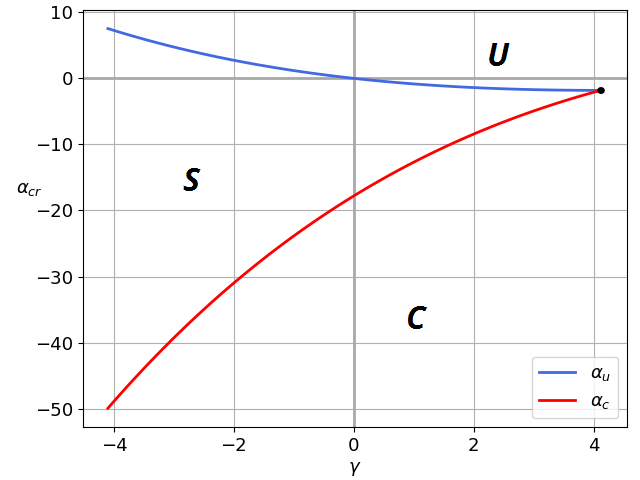
\includegraphics[scale=0.5]{x0=0,00.png} \\ (a) $ x_0 = 0.0 $ }
\end{minipage}
\hspace{5cm}
\begin{minipage}[h]{0.2\linewidth}
\center{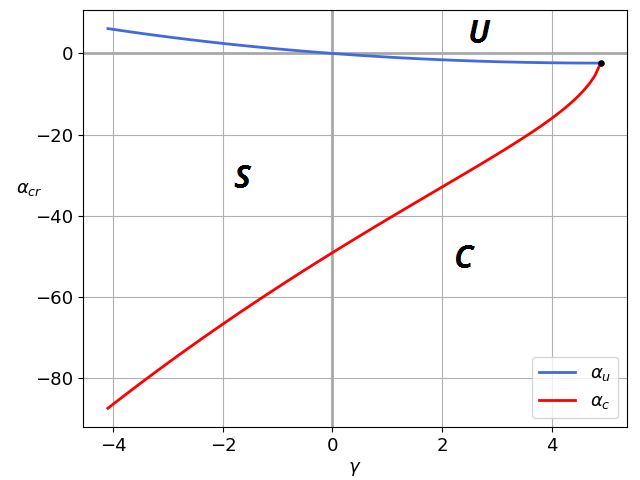
\includegraphics[scale=0.5]{x0=0,33.png} \\ (b) $ x_0 = 0.33 $ }
\end{minipage}
\end{figure}

Кривые $ \alpha_u $ и $ \alpha_c $ являются важнейшими элементами для построения областей значений $ \alpha $ и $ \gamma $, определяющих устойчивость нулевого решения краевой задачи. Так область $ S $ соответствует случаю устойчивого нулевого состояния равновесия, $ U $ -- неустойчивых, симметричных относительно нуля состояний равновесия, а в области параметров $ C $ наблюдается возникновение цикла вокруг нулевого решения краевой задачи.

Кривые $ \alpha_u $ и $ \alpha_c $ пересекаются в точке с отрицательным значением ординаты и абсциссой $ \gamma = \gamma_* $. Для $ x_0 = 0.0 $ $ \gamma_* \approx 4.116 $. С ростом величины $ x_0 $ наблюдается увеличение значения $ \gamma_* $. Так для $ x_0 = 0.33 $ $ \gamma_* \approx 4.896 $. Помимо этого на кривой $ \alpha_u $ можно найти значение $ \hat{\gamma} < \gamma_* $ такое, что для значений $ \hat{\gamma} < \gamma < \gamma_*  \quad d_0 > 0 $, что говорит о грубой потере устойчивости нулевого решения. Для $ x_0 = 0.0 $ $ \hat{\gamma} \approx 4.039 $, а для $ x_0 = 0.33 $ $ \hat{\gamma} \approx 4.772 $.

Для значений $ \gamma > \gamma_* $ сохраняется только кривая $ \alpha_u $, а нулевое состояние равновесия останется неустойчивым.

\newpage

\begin{center}
Критические зависимости параметра $ \alpha $ для $ x_0 \in [x_1, x_2] $, где $ x_2 \approx 0.45 $
\end{center}

\begin{figure}[h]
\begin{minipage}[h]{0.99\linewidth}
\center{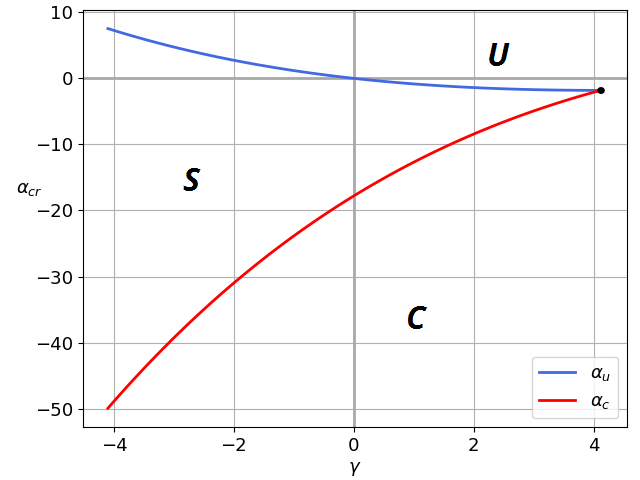
\includegraphics[scale=0.5]{x0=0,00.png} }
\caption{$ x_0 = 0.0 $}
\end{minipage}
\end{figure}

\end{document}